%% ==============
\chapter{Evaluation}
\label{ch:Evaluation}
%% ==============
In this chapter we compare all the techniques we implemented with plain uniform and powerbased Next Event Estimation and with PBRTs implementation. We try to point out the strength and weaknesses of the techniques for certain kind of scenes and scenarios. In this context we mainly argue about image quality, time and memory. We compare time and momery consumtion based on the Mean Squared Error (MSE) metric from equation~\ref{eq:mse}. Where $Y$ is the vector of pixels of length $n$ of our reference image and $\widetilde{Y}_i$ is the vector of pixels of the compared image. 

\begin{align}\label{eq:mse}
\text{MSE} = \frac{1}{n}\sum_{i=1}^{n}(\abs{Y - \widetilde{Y}_i})^2
\end{align}


We compare based on an equal MSE, therefor the MSE is an estimator for our image quality. When we argue about image quality throughout this chapter we rather refer to the perceived image quality\footnote{The MSE in itself has a perception compontent because of the square. The MSE is a very commonly used estimator, nonetheless one could imagine using a metric which does reflect human perception more closely. This usually leads to problems with subjectivity.}, in our case this usually means whether sensible artifacts are present. As all the compared techniques are unbiased, given unlimited time, all of them would converge to the same image. Artifacts are usually areas or edges which will converge very slowly, in practice maybe never. When we say a technique has a bad image quality, we say that artifacts are present. 

\section{Setup}

The test system we used for comparisons is a i7-4790K CPU @ 4GHz, 32 GB RAM, running on Windows 10 64-Bit. Images are produced by PBRT-v3 forked on March 30\footnote{Latest commit before the fork: \url{https://github.com/mmp/pbrt-v3/commit/42c42c194bab970d8adc3f6b5e3afbbc172c3375}}. PNEE techniques are added on top of this fork, the complete implementation can be found at \url{https://github.com/AndiMiko/pbrt-v3}.

\subsection{Problem cases}

We tried to identify problematic light and object constellations, which are causing trouble for various kinds of techniques. The most prominent and comprehensible scenarios are to be covered bellow. 

\begin{description}
    \item[1. High Frequency.] 
    \item[2. Level of Detail.]
    \item[3. High variantion of light power.] 
    \item[4. High number of contributing light sources.]
    \item[5. Non-axis aligned planes.]
    \item[6. Highly occluding planes.]
    \item[7. Tiny but important solid angles.] 
\end{description} 
% which problematic setups we have / we can solve

\subsection{Test scenes}

We designed a special scene, called \textit{Stanford-Museum}, for most of the comparisons we present in this chapter. This scene covers all aforementioned problem cases and thus gives a good impression about strengths and weaknesses of each technique. The simplicity of the scene allows the reader to clearly correlate variance with the problem cases, but ultimately does not provide a photorealistic appeal. On the other hand we present two more scenes, \textit{bathroom} and \textit{measure-one}, for a comparison on real scenes with all sorts of details.

\paragraph{Stanford-Museum}

We describe the most important problem cases we had in mind when designing the Stanford-Museum scene in figure~\ref{fig:stanfordmuseumref}, which is the reference image we calculate the MSE against. The scene contains 4058 light sources, all of whom are point light sources. We chose point light sources, because sampling a point on a light source is not a concern of PNEE, thus reducing variance from other effects does discloses artifacts produced by our techniques more clearly. We also render the scene with a pathtracer with a max depth parameter of one, again, using the same argument, as depth introduces variance from the indirect lighting term of the pathtracer.

\begin{figure}[ht]\centering
\captionsetup[subfigure]{labelformat=empty}

\begin{tikzpicture}[zoomboxarray, zoomboxes below, zoomboxarray inner gap=0.4cm,
zoomboxarray columns=4, zoomboxarray rows=2,remember picture, black and white]
   \node [image node] {
   \setcounter{zoombox}{0} 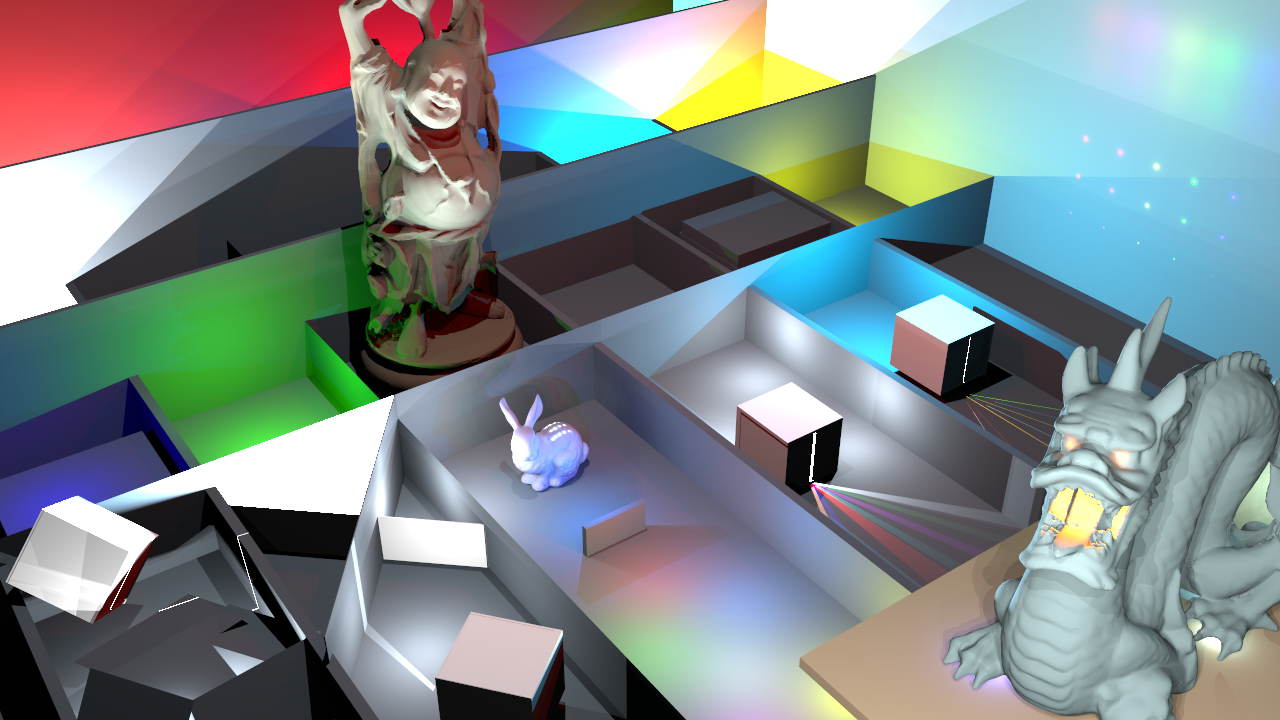
\includegraphics[width=1\textwidth]{figures/StanfordMuseum_ref.png}};
   
   \zoombox[magnification=0.8, color code=red]{0.85,0.3}
   \zoombox[magnification=1.5, color code=yellow]{0.334,0.78}
   
   \zoombox[magnification=2.3, color code=green]{0.767,0.47}
   \zoombox[magnification=1.4, color code=olive]{0.895,0.79}
   
   \zoombox[magnification=2, color code=brown]{0.285,0.32}
   \zoombox[magnification=1.3, color code=blue]{0.11,0.2}
   
   \zoombox[magnification=2, color code=cyan]{0.085,0.63}
   \zoombox[magnification=2, color code=pink]{0.6,0.68}

\end{tikzpicture}
\begin{tikzpicture}[overlay,remember picture]

\foreach \X in {1,...,\thezoombox}
   {\node[anchor=south,yshift=-13pt] at (zoombox-\X.south) 
   {\tiny (\X)};}
   \setcounter{zoombox}{0} 
\end{tikzpicture}

\caption{The reference image for \textit{Stanford-Museum}. }
\begin{tabular}{|c|cc|ccc|}
\hline 
a  & b & c & 1 & 2 & 3 \\\hline
d  & e & f & 4 & 5 & 6 \\
g  & h & i & 7 & 8 & 9 \\\hline
\end{tabular}
\end{figure}

\subsection{Techniques}

% which implementations will be compared

\subsection{Parameter Comparison}




\label{ch:ev:photontree}


\label{ch:ev:cdftree}

% which parameters did we try to configure. Which parameters turned out to be good and will be set as fixed?

\section{Equal time comparisons}

\section{Memory comparisons}

\section{Conclusions}
